% Predictive latent representation and evaluation protocol. Former Section 3
% (Methods), compressed and de-diaried. JFM structure pass: five subsections
% reduced to three (model+objective+conditioning; closure protocol;
% diagnostics/controls/uncertainty), the two run-in \emph headings of the old
% diagnostics subsection rewritten as prose, and the two method schematics
% combined into one figure (architecture + evaluation protocol) with the
% predictive-vs-reconstructive contrast moved to Appendix~\ref{app:reg}.

\subsection{Model, training objective, and conditioning split}
\label{sec:methods_arch}
\label{sec:methods_loss}

The predictive encoder $E_\theta$ maps the mid-plane vorticity field
$\omegaz(192,96)$ to a latent $\zvec \in \mathbb{R}^d$ at $d \in \{16, 32, 64\}$. It
is a hybrid network: three convolutional downsampling stages produce a
$24 \times 12 \times 256$ feature map, a six-layer vision transformer processes
the resulting tokens, and the class-token output is projected to $\zvec$ through
a single linear layer with a batch-normalisation boundary, which the
characteristic-function regulariser below requires. The encoder is
\emph{unconditional} by design: it sees only the flow field, not the gust
parameters $\cvec = (G,D,Y)$. This is the property that lets the latent itself
serve as the observable a controller would have access to, since at deployment
the gust parameters are not known a priori (\S\ref{sec:discussion}). The
conditional predictor, by contrast, still requires $\cvec$, either estimated
from the wall or marginalised over, so an observable latent is a necessary but
not a sufficient condition for a deployable forward model.

The predictor $P_\phi$ advances the latent in time. It is a six-layer
autoregressive transformer with rotary positional embeddings and a causal mask,
conditioned on $\cvec$ through adaptive layer-norm modulation at every block;
its internal structure is given in Appendix~\ref{app:reg}. The predictor is the only stage
that sees $\cvec$. Figure~\ref{fig:method}(a) shows the encoder and
predictor, and panel~(b) sets out the matched-predictor evaluation protocol used
throughout; the contrast between the predictive training signal and the
reconstructive one, in which the reconstructive autoencoder passes the field at
time $t$ through an encoder and a decoder and incurs a field-space error whereas
the predictive model encodes the fields at $t$ and $t+\Delta t$ with shared
weights and incurs a latent-space error between the predicted and observed target
embeddings, with no field-space loss, is drawn in Appendix~\ref{app:reg}
(figure~\ref{fig:predictive_vs_reconstructive}).
Table~\ref{tab:architecture} summarises the two networks.

\begin{table}
  \centering
  \caption{Encoder and predictor configuration. The encoder is unconditional;
  the gust parameters $\cvec = (G,D,Y)$ enter only
  the predictor, through identity-initialised adaptive layer normalisation
  (AdaLN-Zero). Parameter counts are for the $d = 64$ configuration; two small
  auxiliary heads read observables off the encoder output during training (a lift
  head, $4\times10^{3}$ parameters, and an $80$-dimensional wake-spectrum head,
  $3.5\times10^{4}$ parameters; \S\ref{sec:methods_loss}).}
  \label{tab:architecture}
  \small
  \fittab{\begin{tabular}{l l l}
    \toprule
     & Encoder $E_\theta$ & Predictor $P_\phi$ \\
    \midrule
    role            & field $\to$ latent (unconditional) & latent dynamics (conditioned) \\
    input           & $\omegaz \in \mathbb{R}^{192 \times 96}$ & latent sequence $\zvec_{1:t}$ \\
    backbone        & 3 conv.\ stages $+$ 6-layer ViT & 6-layer autoregressive transformer \\
    width / heads   & $256$ / $8$ & $384$ / $16$ \\
    tokens / context & $24 \times 12 = 288$ spatial & $\le 32$ temporal (causal) \\
    conditioning    & none & AdaLN-Zero on $\cvec = (G,D,Y)$, rotary time \\
    latent read-out & class token $\to$ linear $\to$ BatchNorm & next-step latent \\
    parameters      & $6.7$M & $16.2$M \\
    \bottomrule
  \end{tabular}}
\end{table}

The predictive encoder and predictor are trained jointly on a one-step
latent-prediction term, a scheduled-sampling rollout term that exposes the
predictor to its own errors, and an anti-collapse regulariser that prevents the
encoder from collapsing to a constant. We use the characteristic-function
regulariser of \citet{lejepa,lewm}, which matches the latent distribution to an
isotropic Gaussian through a small number of random projections, with an
automatic fall-back to a variance-covariance objective \citep{vicreg} should the
participation ratio of the latent indicate collapse. Its configuration is given
in Appendix~\ref{app:reg}.

Two auxiliary heads read aerodynamic observables off the encoder output during
training: a lift head that maps $\zvec_t$ to $C_L(t)$, and a wake head that maps
$\zvec_t$ to an $80$-dimensional signed wake spectrum, both trained with small
weights jointly with the representation and neither part of the latent-prediction
loss. These heads are adopted from the observable-augmentation
lineage \citep{fukami2023,fukami2025}. They are also, however, the reason the
present predictive encoder is not a clean isolation of the training objective:
the reconstructive baseline below carries a lift head but not a wake head, and
the two encoders differ in architecture as well. We are explicit about this
throughout. The headline comparison is therefore between encoder
\emph{families} as configured, and the controls of \S\ref{sec:res_controls}
are designed to separate the objective from the architecture and the wake
supervision.

\begin{figure}
  \centering
  \begin{subfigure}{\linewidth}
    \centering
    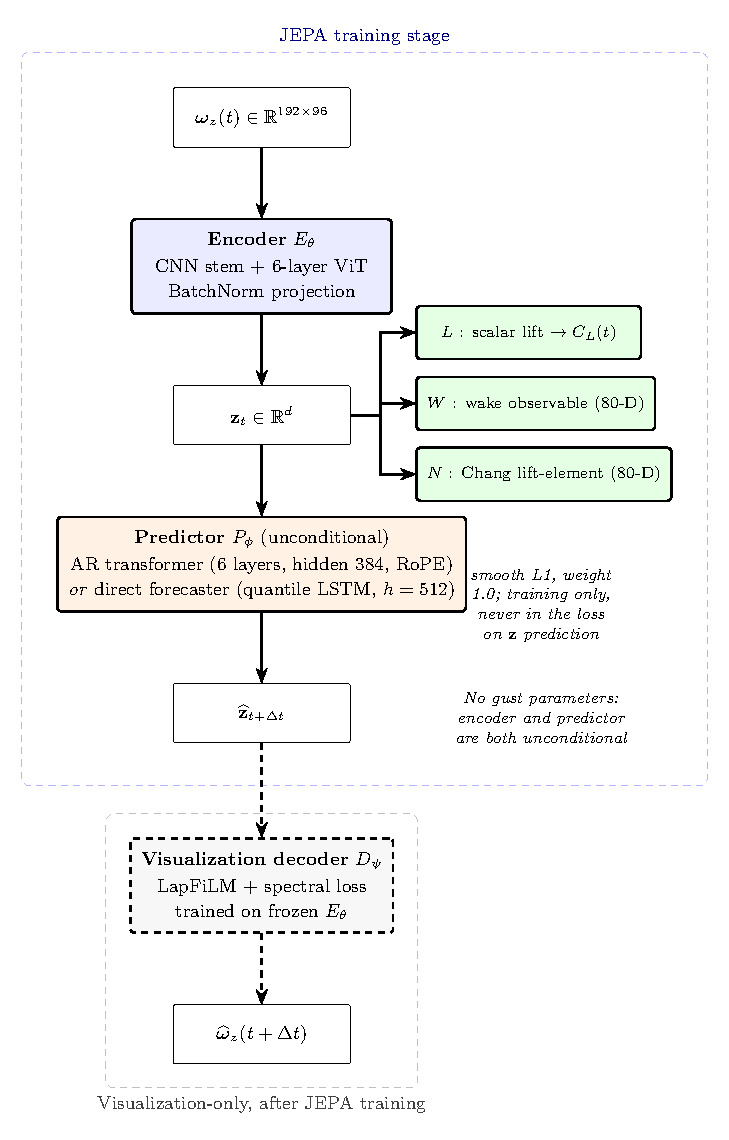
\includegraphics[width=0.52\linewidth]{sections/figures/tikz/fig1_jepa_architecture.pdf}
    \caption{}
    \label{fig:method_arch}
  \end{subfigure}
  \\[1.5ex]
  \begin{subfigure}{\linewidth}
    \centering
    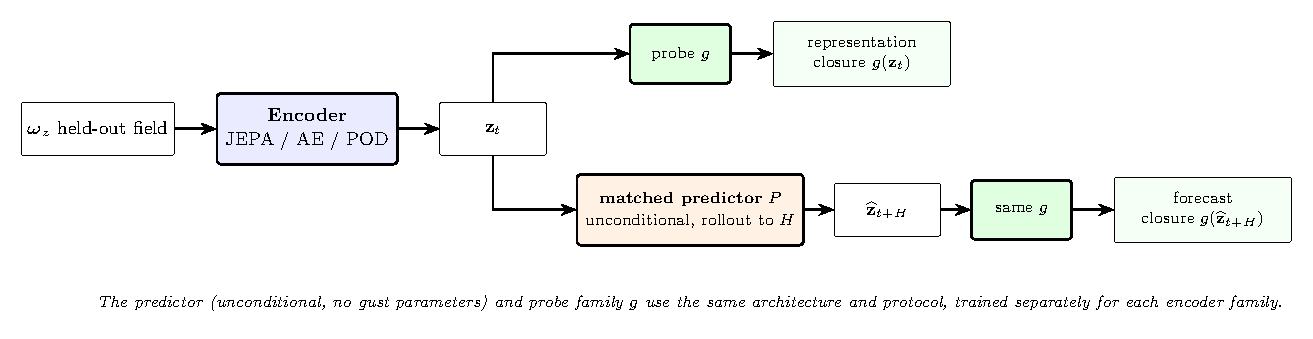
\includegraphics[width=0.98\linewidth]{sections/figures/tikz/fig_eval_protocol.pdf}
    \caption{}
    \label{fig:method_eval}
  \end{subfigure}
  \caption{The predictive model and how it is evaluated. (a) The encoder is
  unconditional and maps the mid-plane vorticity field to a latent $\zvec_t$,
  while the autoregressive predictor advances the latent given the gust
  conditioning $\cvec = (G,D,Y)$, which enters the predictor alone. The two
  auxiliary observable heads (lift and wake) read $\zvec_t$ during JEPA training
  with small weights and are not part of the latent-prediction loss; they are
  omitted from the schematic for clarity. The visualisation decoder is trained
  only after the encoder is frozen and is used solely for the diagnostic decodes
  of \S\ref{sec:res_physical}, never in the predictive loss. (b) Evaluation
  applies the same predictor architecture, conditioning, and probe family $g$, each
  trained or fitted separately per encoder family: a probe on the simulation-encoded
  latent measures representation
  closure, and the same probe on the rolled-out latent $\widehat{\zvec}_{t+H}$
  measures forecast closure.}
  \label{fig:method}
\end{figure}

\subsection{Matched-predictor closure protocol}
\label{sec:methods_protocol}
\label{sec:methods_closure}

The comparison rests on a single principle: every baseline is the same
three-stage pipeline, and only the encoder differs. Each encoder produces a
latent trajectory $\zvec_{1:T}$ from the vorticity fields; an identical
autoregressive transformer predictor rolls it forward one step at a time given
$\cvec$; and an identical probe family maps the predicted latent to a physical
observable for evaluation (figure~\ref{fig:method}(b)). The predictor
architecture, its training recipe, the parametric conditioning, and the probe
family are held fixed across the three encoder families. The latent dimension
is matched within each family: JEPA at $d \in \{16, 32, 64\}$, the reconstructive
autoencoder at $d \in \{3, 32, 64\}$ to include both the published $d = 3$
recipe and matched-capacity variants, and POD at $d \in \{16, 32, 64\}$. The
predictive family is additionally swept to $d \in \{4, 8\}$ and ablated without its
predictor conditioning in \S\ref{sec:res_controls}. This
isolation is the only fair way to attribute forecast quality to the
representation rather than to incidental differences in the predictor or its
training. The reconstructive autoencoder uses its best-documented configuration,
with ReLU activations, group normalisation, and a future-lift head at horizons
$\{8, 16, 24\}$, rather than the strict published variant (tanh, no normalisation,
a current-lift head), which we found gives a worse parametric probe; the
comparison is therefore against a tuned baseline, not a hobbled one.

The figure of merit is forward physical closure, the empirical test of the
geometric criterion set out in the introduction: a latent whose metric stays
aligned with the transport geometry under the predictor keeps each observable
recoverable along the rollout, while one that drifts off the manifold loses it. Given a ground-truth
$\cvec$ and an initial latent, the predictor is rolled recursively to $H = 16$, and
at each step the probe maps the predicted latent to each observable. A small
closure error means the encoder produces a latent whose dynamics, propagated by
the predictor, retain the information the probe needs to recover the
physical quantity; a large error means either that the encoder discarded that
information or that the predictor lost it during rollout, a distinction the
drift diagnostic below resolves. We report closure on the held-out test\_b and
test\_c encounters as the mean absolute error against the simulation, with
bootstrap $95\%$ confidence intervals over encounters and the coefficient of
determination $R^2$.
%
% HONESTY NOTE: the original draft headed the results with a *training-set* R^2
% (mean 0.835). That number is retained only as a training-fit reference
% (table~\ref{tab:b1_closure_train_r2}); the headline is the held-out error.
% test_b / test_c R^2 computed from the same rollout predictions used for the
% held-out MAE and reported in table~\ref{tab:closure} panel (b) (forecast) and
% panel (a) (representational closure).
The held-out forecast $R^2$ (Markov rollout at $H = 16$) is reported in
table~\ref{tab:closure}(b), and the representational closure (probe on the
simulation-encoded latent) in table~\ref{tab:closure}(a).

\subsection{Diagnostics, controls, and uncertainty}
\label{sec:methods_diag}

Two diagnostics turn the closure number into a mechanism. The first is the
latent drift, which addresses the fact that a predictor with low one-step error
need not produce a useful long rollout, because each prediction is fed back as
the next input and small geometric errors accumulate. We quantify how far a
rollout has left the training manifold by the Mahalanobis distance of the
rolled-out latent at horizon $H$, measured against the distribution of
simulation-encoded latents for the same encoder, normalised by the Mahalanobis
distance of the simulation-encoded latent itself. A ratio near one means the
rollout stays within the natural spread of the training latents; a large ratio
means it has gone out of distribution, so that the probe is then queried outside
its support.

The second diagnostic is a conditioning-only floor. Because the predictor is
conditioned on $\cvec = (G,D,Y)$, a natural concern is that the forecast quality
is carried by the conditioning rather than by the latent. We bound this with a
kernel-ridge regressor that maps $\cvec$ directly to each observable at the
forecast horizon $H = 16$, with no latent input, fit on training and evaluated on
the held-out splits, so that it is frame-matched to the closure it is compared
against. This is the floor any learned encoder must clear at that horizon to
demonstrate that its latent contributes beyond what is already implicit in the
parameters. At the impact frame the same parameter floor is high, because the
just-released gust nearly determines the instantaneous state; the predictive
latent must instead close the gap that opens as the wake evolves
(\S\ref{sec:res_closure}).

Because the predictive encoder differs from the reconstructive baseline in
objective, architecture, and auxiliary supervision at once, the comparison is
accompanied by controls that vary one factor at a time: a crossing of objective
with architecture at matched auxiliary heads, an ablation of each auxiliary head,
and an ablation of the predictor conditioning (\S\ref{sec:res_controls}). Every
held-out $R^2$ and mean absolute error reported below carries three independent
uncertainty signals, following the reporting protocol fixed with the data split:
a $2000$-resample bootstrap over the held-out encounters, the standard deviation
across three encoder retrains from independent seeds, and a five-fold
cross-validation over cases on the probe read-out. Their full specification is in
Appendix~\ref{app:reg}.
